% !TEX root = ../axiomatic.tex

\section{Proof} \label{sec: proof}

In this section we prove Theorem \ref{theorem: main}. We do so by establishing a linearly dual version stated as Theorem \ref{theorem: main reformulated}. The first subsection is devoted to formulating this dual version. The second reinterprets the freeness axiom in this language. The third establishes the base case of an induction. The fourth explores the relationship between the dual version of the cup-$i$ products and the boundary map of simplicial sets and the final subsection carries out the induction argument proving the theorem.

\subsection{Dual version}

\begin{lemma} \label{lemma: cup-i constructions and diagonals are the same}
	Let $C^* = \Hom_{\F}(C_*, \F)$ with $C_*$ a finite dimensional chain complex. The linear duality functor induces a bijection between cup-$i$ structures on $C^*$ and $\F[\Sigma_2]$-linear chain maps $W \to \Hom_{\F}(C_*, C_*^{\tensor 2})$.
\end{lemma}

\begin{proof}
    Since $C_\ast$ is finite dimensional, we have
    \[
    \Hom_{\F}(C_\ast, C_\ast^{\otimes 2}) \cong \Hom_{\F}((C^\ast)^{\otimes 2}, C^\ast).
    \]
    Therefore, the hom-tensor adjunction gives
    \begin{align*}
    \Hom_{\F[\Sigma_2]}\big(W, \Hom_{\F}(C_\ast, C_\ast^{\otimes 2}) \big) & \cong
    \Hom_{\F[\Sigma_2]}\big(W, \Hom_{\F}((C^\ast)^{\otimes 2}, C^\ast) \big) \\ & \cong
    \Hom_{\F} \big(W \otimes_{\F[\Sigma_2]} (C^\ast)^{\otimes 2}, C^\ast \big)
    \end{align*}
    as chain complexes of $\F$-modules.
\end{proof}

\begin{definition}
	Let $\mathcal Z(2)$ be the universal chain complex of $\F[\Sigma_2]$-modules together with a natural $\F[\Sigma_2]$-linear chain maps
	\[
	\mathcal Z(2) \to \Hom_{\F}\big( N_\bullet(X), N_\bullet(X)^{\otimes 2} \big)
	\]
	for every simplicial set $X$.
\end{definition}

According to Lemma \ref{lemma: cup-i constructions and diagonals are the same} a cup-$i$ construction is equivalent to a natural collection of $\F[\Sigma_2]$-linear chain maps
\[
W \to \Hom_{\F}\big( N_\bullet(X), N_\bullet(X)^{\otimes 2} \big)
\]
which, by the universality of $\mathcal Z(2)$, is equivalent to an $\F[\Sigma_2]$-linear chain map
\[
W \to \mathcal Z(2).
\]
We will reference a cup-$i$ construction and to its associated $\F[\Sigma_2]$-linear chain map $\triangle \colon W \to \mathcal Z(2)$ interchangeably, denoting $\triangle(e_i)$ simply by $\triangle_i$.

We can give a more explicit description of $\mathcal Z(2)$ by noticing that a natural transformation
\[
f_X \colon N_\bullet(X) \to N_\bullet(X)^{\otimes 2}
\]
is determined by the images, for each $n \in \N$, of the elements $\id_{[n]} \in N_\bullet(\simplex^n)$, and, conversely, that a set containing an element $f(\id_{[n]})$ in $N_\bullet(\simplex^n)^{\otimes 2}$ for each $n \in \N$ defines a natural transformation $f_X$ if and only if the induced maps $f_{\simplex^n}$ satisfy
\[
\begin{tikzcd}
N_\bullet(\simplex^n) \arrow[r, "f_{\simplex^n}"] \arrow[d, "(s_j)_\ast"] & N_\bullet(\simplex^n)^{\otimes 2} \arrow[d, "(s_j)_\ast^{\otimes 2}"] \\
N_\bullet(\simplex^{n-1}) \arrow[r, "f_{\simplex^{n-1}}"] & N_\bullet(\simplex^{n-1})^{\otimes 2}
\end{tikzcd}
\]
for each $j = 0, \dots, n$. That is to say, if
\begin{equation} \label{equation: naturality and degeneracy}
(s_j)_\ast^{\otimes 2} \big( f(\id_{[n]}) \big) = 0
\end{equation}
for each $j = 0, \dots, n$. We record the following direct consequence for later reference:

\begin{lemma} \label{lemma: condition to be in the kernel of s}
	A basis element $\delta_V \otimes \delta_W$ is in the kernel of $(s_j)^{\otimes 2}_\ast$ if and only if both $j$ and $j+1$ are missing from either $V$ or $W$.
\end{lemma}

\begin{definition}
	Let $\Delta \colon W \to \mathcal Z(2)$ be the $\F[\Sigma_2]$-linear map defined by
	\[
	\Delta_i(\id_{[n]}) = \sum_{\P_{n-i}(n)} \delta_{U^{-}} \otimes \delta_{U^{+}}
	\]
	for $i \leq n$ and $\Delta_i(\id_{[n]}) = 0$ otherwise.
\end{definition}

We now state an equivalent formulation of Theorem \ref{theorem: main}

\begin{theorem} \label{theorem: main reformulated}
	If $\triangle : W \to \mathcal{Z}(2)$ is a free non-degenerate cup-$i$ construction, then, for every $i \geq 0$, either $\triangle_i = \Delta_i$ or $\triangle_i = T \Delta_i$.
\end{theorem}

For the rest of Section \ref{sec: proof} we take $\triangle$ to be a free and non-degenerate cup-$i$ construction.

\subsection{Freeness revisited}

The freeness of $\triangle$ can be expressed via the following
\begin{lemma} \label{lemma: freeness recasted}
	If
	\[
	\triangle_i(\id_{[n]}) = \sum_{\Lambda} \delta_{V_\lambda} \otimes \delta_{W_\lambda}
	\]
	for some $i < n$, then
	\[
	\delta_{V_{\lambda_1}} \otimes \delta_{W_{\lambda_1}} \neq
	\delta_{W_{\lambda_2}} \otimes \delta_{V_{\lambda_2}}
	\]
	for every $\lambda_1, \lambda_2 \in \Lambda$.
\end{lemma}

A consequence of this lemma is

\begin{lemma} \label{lemma: (1+T) triangle = 0 implies triangle = 0}
    If
    \[
    (1 + T) \triangle_i(\id_{[n]}) = (1 + T) \sum_{\Lambda} \delta_{V_\lambda} \otimes \delta_{W_\lambda}
    \]
    for some $i < n$, then there exists a partition of $\Lambda = \Lambda_1 \sqcup \Lambda_2$ such that
    \begin{equation} \label{equation: splitting after 1+T}
    \triangle_i(\id_{[n]}) = \sum_{\Lambda_1} \delta_{V_\lambda} \otimes \delta_{W_\lambda} + \sum_{\Lambda_2} \delta_{W_\lambda} \otimes \delta_{V_\lambda}.
    \end{equation}
\end{lemma}

\begin{proof}
	We directly have that \eqref{equation: splitting after 1+T} holds up to an element in the kernel of $(1+T)$. This kernel is generated by elements of the form $\delta_U \otimes \delta_U$ and $\delta_V \otimes \delta_W + \delta_W \otimes \delta_V$. Therefore, Lemma \ref{lemma: freeness recasted} implies the element in the kernel must be $0$.
\end{proof}

\subsection{Special cases}

In this subsection we prove Theorem \ref{theorem: main reformulated} for all pairs of integers satisfying $i > n-2$.

\begin{lemma}
	If $i > n$ then $\triangle_i(\id_{[n]}) = 0$.
\end{lemma}

\begin{proof}
	This is immediate since $\chains(\simplex^n)^{\otimes 2}_i = 0$ in this range.
\end{proof}

\begin{lemma} \label{lemma: triangle_n of n = n x n}
    For any $n \in \N$
    \[
    \triangle_n(\id_{[n]}) = \id_{[n]} \otimes \id_{[n]}.
    \]
\end{lemma}

\begin{proof}
	For any $n \in \N$, the vector space $\chains(\simplex^n)^{\otimes 2}_n$ is one dimensional and either $\triangle_n(\id_{[n]}) = 0$ or $\triangle_n(\id_{[n]}) = \id_{[n]} \otimes \id_{[n]}$. If the desired conclusion does not hold, there exists $n \in \N$ smallest such that $\triangle_n (\id_{[n]}) = 0$. If $n > 0$ then
    \begin{align*}
    (1 + T) \triangle_{n-1}(\id_{[n]}) =
    \partial \triangle_{n}(\id_{[n]}) + \triangle_{n}(\partial\, \id_{[n]}) =
    0,
    \end{align*}
    and Lemma \ref{lemma: (1+T) triangle = 0 implies triangle = 0} implies $\triangle_{n-1}(\id_{[n]}) = 0$. From this and the assumption
    \[
    \triangle_{n-1} (\id_{[n-1]}) = \id_{[n-1]} \otimes \id_{[n-1]}
    \]
    we obtain
    \begin{equation}
    \begin{split}
    (1+T)\triangle_{n-2}(\id_{[n]}) =
    \partial \triangle_{n-1}(\id_{[n]}) + \triangle_{n-1}(\partial \id_{[n]}) =
    \sum_{u = 0}^n \delta_u \otimes \delta_u,
    \end{split}
    \end{equation}
 	which is a contradiction since $\sum \delta_u \otimes \delta_u$ is not in the image of $(1+T)$.

    The previous argument shows that $\triangle_n(\id_{[n]}) = 0$ for every $n \in \N$. This serves as the base case of an induction argument in $n-i$ proving that $\triangle_i(\id_{[n]}) = 0$ for every $i, n \in \N$. For the induction step, consider
    \begin{align*}
    (1+T) \triangle_{i-1}(\id_{[n]}) =
    \partial \triangle_{i}(\id_{[n]}) + \triangle_{i}(\partial\, \id_{[n]}) =
    0,
    \end{align*}
    which, by Lemma \ref{lemma: (1+T) triangle = 0 implies triangle = 0}, implies $\triangle_{i-1} (\id_{[n]}) = 0$.
\end{proof}

\begin{lemma}
	For $n \geq 1$, either $\triangle_{n-1}(\id_{[n]})$ or $T \triangle_{n-1}(\id_{[n]})$ is equal to
	\[
	\sum_{\substack{u \leq n \\ u \text{ odd }}} \delta_u \otimes \id_{[n]} \ + \sum_{\substack{u \leq n \\ u \text{ even }}} \id_{[n]} \otimes \delta_u.
	\]
\end{lemma}

\begin{proof}
	Since $\triangle_{n}(\id_{[n]}) = \id_{[n]} \otimes \id_{[n]}$ and $\triangle_{n}(\partial\, \id_{[n]}) = 0$ we have
	\[
	(1+T) \triangle_{n-1}(\id_{[n]}) = (1 + T) \sum_{k = 0}^n \delta_u \otimes \id_{[n]}
	\]
	and we need to show that the partition provided by Lemma \ref{lemma: (1+T) triangle = 0 implies triangle = 0} is that of even and odd non-negative integers less than $n$. Let us argue by contradiction and assume some $j$ and $j+1$ belong to the same subset in the partition. With out loss of generality we have
	\[
	\triangle_{n-1}(\id_{[n]}) = (\delta_j + \delta_{j+1}) \otimes \id_{[n]} + O(j, j+1)
	\]
	where $O(j, j+1)$ is an element in the span of basis elements missing both $\delta_j$ and $\delta_{j+1}$ from both of its tensor factors. Since $\triangle_{n-1}(\partial\, \id_{[n-1]}) = \sum_{k=0}^n \delta_k \otimes \delta_k$,
	\[
	(1+T) \triangle_{n-2}(\id_{[n]}) = (1+T)(\delta_j \otimes \delta_{j+1}) + P(j, j+1)
	\]
	where $P(j, j=1)$ is an element in the span of basis elements with $j$ and $j+1$ missing from at least one of its tensor factors. Using Lemma \ref{lemma: (1+T) triangle = 0 implies triangle = 0} and Lemma \ref{lemma: condition to be in the kernel of s} we get a contradiction since $\delta_j \otimes \delta_{j+1}$ is not in the kernel of $(s_j)_\ast^{\otimes 2}$.
\end{proof}

\subsection{Boundaries and coproducts}

\begin{notation}
	Given $\xi : \P_{n-i}(n) \to \{-, +\}$ we denote by $\bar{\xi}$ the function with the same domain and range satisfying $\xi \neq \bar{\xi}$ pointwise, and simplify the notation $U^{\xi(U)}$ and $U^{\bar{\xi}(U)}$ to $U^\xi$ and $U^{\bar{\xi}}$ respectively.
\end{notation}

A direct consequence of Lemma \ref{lemma: (1+T) triangle = 0 implies triangle = 0} is the following

\begin{lemma} \label{lemma: (1+T) triangle = (1+T) sum implies triangle = sum}
    If
    \[
    (1 + T) \triangle_i (\id_{[n]}) =
    (1 + T) \sum_{\P_{n-i}(n)} \delta_{U^-} \otimes \delta_{U^+}
    \]
    for some $i < n$, then there exists $\xi : \P_{n-i}(n) \to \{-, +\}$  such that
    \[
    \triangle_i (\id_{[n]})\ =\! \sum_{\P_{n-i}(n)} \delta_{U^{\xi}} \otimes \delta_{U^{\bar{\xi}}}.
    \]
\end{lemma}

\begin{notation}
    For $U \in \P_{n-i}(n)$ we write $u \notin U$ if $u \in \{0 < \cdots< n\} \setminus U$. If $u \notin U$ define $u.U = \{u\} \union U \in \P_{n-i+1}(n)$ and if $u \in U$ define $U \setminus u = U \setminus \{u\} \in \P_{n-i-1}(n)$.
\end{notation}

\begin{lemma} \label{lemma: boundary of triangle}
	If for some $i < n$ there exists $\xi : \P_{n-i}(n) \to \{-, +\}$ such that
	\[
	\triangle_i(\id_{[n]})\ =\! \sum_{\P_{n-i}(n)} \delta_{U^{\xi}} \otimes \delta_{U^{{\bar{\xi}}}}
	\]
	then
	\begin{align}
	\label{equation: boundary of triangle}
	\partial \triangle_i(\id_{[n]})\ = &
	\sum_{\P_{n-i}(n)} \left( \, \sum_{u \in U^{\bar{\xi}}} \delta_{u.U^\xi} \tensor \delta_{U^{\bar{\xi}}} \ +
	\sum_{u \in U^\xi} \delta_{U^\xi} \tensor \delta_{u.U^{\bar{\xi}}} \right) \\ + &
	\sum_{\P_{n-i}(n)} \sum_{x \notin U} \left( \delta_{x.U^-} \tensor \delta_{U^+}\ +\ \delta_{U^-} \tensor \delta_{x.U^+} \right).
	\end{align}
\end{lemma}

\begin{proof}
	We use the cosimplicial identity $\delta_q \delta_p = \delta_{p-1} \delta_q$ for $p \geq q$ to establish
	\begin{equation} \label{equation: partial of d over P}
	\partial \! \sum_{\P_{n-i}(n)} \delta_{U}\ =\ \sum_{k = 0}^{i} \sum_{\P_{n-i}(n)} \delta_{U} \delta_k \ = \sum_{\P_{n-i}(n)} \sum_{u \not\in U} \delta_{u.U}
	\end{equation}
	from which identity \eqref{equation: boundary of triangle} follows directly.
\end{proof}

\begin{lemma} \label{lemma: boundary of triangle}
	If for some $i \leq n$
	\[
	\triangle_i(\id_{[n-1]})\ =\! \sum_{\P_{n-i-1}(n)} \delta_{U^-} \otimes \delta_{U^+}
	\]
	then
	\begin{align}
	\label{equation: triangle of boundary}
	\triangle_i (\partial \, \id_{[n]}) \ =\! \sum_{\P_{n-i}(n)} \left( \,
	\sum_{u \in U^+} \delta_{u.U^-} \tensor \delta_{U^+} \ +
	\sum_{u \in U^-} \delta_{U^-} \tensor \delta_{u.U^+} \right).
	\end{align}
\end{lemma}

\begin{proof}
	Let
	\begin{align*}
	& S_1 = \big\{(u, V)\ |\ V \in \P_{n-1-i}(n-1) \text{ and }  u \in \{0, \dots, n \} \big\}, \\
	& S_2 = \big\{(w, W)\ |\ W \in \P_{q}(n) \text{ and } w \in W \big\}
	\end{align*}
	and notice that identity \eqref{equation: triangle of boundary} is equivalent to
	\begin{equation} \label{equation: triangle of partial recasted}
	\sum_{(u, V) \in S_1} \delta_{V^\xi}\delta_u \otimes \delta_{V^{\bar{\xi}}}\delta_u \ \, =
	\sum_{\substack{(w, W) \in S_2 \\ w \in W^{\bar{\xi}}}} \delta_{w.W^\xi} \tensor \delta_{W^{\bar{\xi}}} \ + \!
	\sum_{\substack{(w, W) \in S_2 \\ w \in W^\xi}} \delta_{W^\xi} \tensor \delta_{w.W^{\bar{\xi}}.}
	\end{equation}
	Define $S_1 \to S_2$ by sending $\big(u, \, \{v_1 < \cdots < v_{q-1}\} \big)$ to $\big(u,\, \{w_1 < \cdots < w_{q}\} \big)$ with
	\[
	w_i =
	\begin{cases}
	v_i & \text{ if } v_i < u \\
	u & \text{ if } v_i < u \leq v_{i+1} \\
	v_{i-1}+1 & \text{ if } v_i < u.
	\end{cases}
	\]
	This function is a bijection since it is injective and both sets have the same cardinality. To establishes \eqref{equation: triangle of partial recasted} we use the simplicial identities to notice that
	\[
	\delta_{V^\xi} \delta_u \otimes \delta_{V^{\bar{\xi}}} \delta_u =
	\begin{cases}
	\delta_{w.W^\xi} \tensor \delta_{W^{\bar{\xi}}} & \text{ if } w \in W^{\bar{\xi}}, \\
	\delta_{W^\xi} \tensor \delta_{w.W^{\bar{\xi}}} & \text{ if } w \in W^\xi.
	\end{cases}
	\]
	if $(u, V) \mapsto (w, W)$.
\end{proof}

\begin{lemma} \label{lemma: boundary gives the lower case}
	For $i \leq n$
	\begin{equation} \label{lemma4: existence: eq1}
	\sum_{U \in \P_{n-i}(n)} \sum_{x \notin U} (\delta_{x.U^-} \tensor \delta_{U^+}\ +\ \delta_{U^-} \tensor \delta_{x.U^+})\ = \
	(1+T) \!\! \sum_{\P_{n-i+1}(n)} \delta_{U^-} \tensor \delta_{U^+.}
	\end{equation}
\end{lemma}

\begin{proof}
	For $U = (u_1, \dots, u_{n-i}) \in \P_{n-i}(n)$ and $x \notin U$ define when possible:
	\begin{align*}
	V_{U,x} = x.U \setminus l_{U, x} & \ \text{ with } l_{U,x} = \max\{u\in U\ |\ x>u\}, \\
	W_{U,x} = x.U \setminus r_{U, x} & \ \text{ with } r_{U,x} = \max\{u \in U\ |\ x>u\}.
	\end{align*}
	Notice that $(l_{U,x}).V_{U,x} = x.U = (r_{U,x}).W_{U,x}$ and that for any $u \in U \setminus \{l_{U,x}, r_{U,x}\}$ we have $\ind_{V_{U,x}}(u) = \ind_{U}(u) = \ind_{W_{U,x}}(u)$.

	We introduce the following sets using tabbing to represent inclusion:

	\vspace*{5pt}
	$L = \{x.U^- \tensor U^+\ | \ U \in \P_{n-i}(n),\ x \notin U\}$
	\vspace*{1pt}
	\begin{tab}
		$L^{e} = \{x.U^- \tensor U^+ \in L\ | \ \ind_{x.U}(x) \text{ even}\}$
		\begin{tab}
			$L_{min}^{e} = \{x.U^- \tensor U^+ \in L^e\ | \ x < u_1 \}$ \par
			$\overline{L}_{min}^{e} = L^{e} \setminus L_{min}^{e}$
			\begin{tab}
				$\overline{L}_{min}^{e,e} = \{ x.U^- \tensor U^+ \in \overline{L}_{min}^{e}\ | \ \ind_{x.U}(l_{U,x}) \text{ even} \}$ \par
				$\overline{L}_{min}^{e,o} = \{ x.U^- \tensor U^+ \in \overline{L}_{min}^{e}\ | \ \ind_{x.U}(l_{U,x}) \text{ odd} \}$
				\vspace*{7pt}
			\end{tab}
		\end{tab}
		$L^{o} = \{x.U^- \tensor U^+\ | \ \ind_{x.U}(x) \text{ odd}\}$ \par
		\begin{tab}
			$L_{max}^{o} = \{x.U^- \tensor U^+ \in L^o\ | \ u_q < x \}$ \par
			$\overline{L}_{max}^{o} = L^{o}\setminus L_{max}^{o}$.
			\begin{tab}
				$\overline{L}_{max}^{o,e} = \{ x.U^- \tensor U^+ \in \overline{L}_{max}^{o}\ | \ \ind_{x.U}(r_{U,x}) \text{ even} \}$ \par
				$\overline{L}_{max}^{o,o} = \{ x.U^- \tensor U^+ \in \overline{L}_{max}^{o}\ | \ \ind_{x.U}(r_{U,x}) \text{ odd} \}$.
			\end{tab}
		\end{tab}
	\end{tab}

	\vspace*{5pt}
	Similar subsets of $R = \{U^-\tensor x.U^+\ | \ U \in \P_{n-i}(n),\ x \in \overline{U}\}$ are defined analogously, and we claim the following four identities:
	\begin{equation}\label{lemma4: existence: eq2}
	\overline{R}_{min}^{o,o} = \overline{L}_{max}^{o,o}\ , \qquad \overline{R}_{min}^{o,e} = \overline{R}_{max}^{e,o}\ , \qquad
	\overline{L}_{min}^{e,o} = \overline{L}_{max}^{o,e}\ , \qquad \overline{L}_{min}^{e,e} = \overline{R}_{max}^{e,e}.
	\end{equation}
	We show only the proof of the first one. The other three are proven analogously.
	\begin{alignat*}{2}
	&\boxed{x.U^-\tensor U^+ \in \overline{L}_{max}^{o,o}}\ &\Longrightarrow\ &\boxed{x.U^-\tensor U^+ =\, W_U(x)^-\tensor r_{U,x}.W_{U,x}^+ \in \overline{R}_{min}^{o,o} \! } \\
	&\boxed{U^-\tensor x.U^+ \in \overline{R}_{min}^{o,o}}\ &\Longrightarrow\ &\boxed{U^-\tensor x.U^+ =\, l_{U,x}.V_U(x)^-\tensor V_{U,x}^+ \in \overline{L}_{max}^{o,o} \ \ }
	\end{alignat*}
	The identities in (\ref{lemma4: existence: eq2}) imply
	\begin{equation} \label{lemma4: existence: eq3}
	\sum_{\overline{L}_{max}^{o},\, \overline{L}_{min}^{e}} d_{x.U^-} \tensor d_{U^+}\ \ +
	\sum_{\overline{R}_{max}^{e},\, \overline{R}_{min}^{o}} d_{U^-} \tensor d_{x.U^+}\ =\ 0.
	\end{equation}
	Let us now consider the right hand side of (\ref{lemma4: existence: eq1})
	\[
	(1+T) \sum_{U \in \P_{n-i+1}(n)} \delta_{U^-} \tensor \delta_{U^+} \, = \!\!
	\sum_{L^0_{max},\, L^r_{min}} \delta_{x.U^-} \tensor \delta_{U^+}\ + \!
	\sum_{R^e_{max}, \, R^o_{min}} \delta_{U^-} \tensor \delta_{x.U^+,}
	\]
	Thanks to (\ref{lemma4: existence: eq3}), the above expression is equivalent to
	\[
	(1+T) \sum_{U \in \P_{n-i+1}(n)} \delta_{U^-} \tensor \delta_{U^+} \, = \
	\sum_{L} \delta_{x.U^-} \tensor \delta_{U^+}\ + \
	\sum_{R} \delta_{U^-} \tensor \delta_{x.U^+.}
	\]
	as claimed.
\end{proof}

\begin{corollary}
	The map $\Delta \colon W \to \mathcal Z(2)$ is a free, non-degenerate Steenrod construction.
\end{corollary}

\begin{proof}
	...
\end{proof}

\subsection{Induction step}

\begin{lemma}
     If for some $i \leq n - 2$ there exists $\xi : \P_{n-i}(n) \to \{-, +\}$ such that
     \[
     \triangle_i(\id_{[n]})\ =\! \sum_{\P_{n-i}(n)} \delta_{U^{\xi}} \otimes \delta_{U^{{\bar{\xi}}}}
     \]
     then,
     \begin{align*}
     \triangle_i(\id_{[n-1]}) = \Delta_i(\id_{[n-1]})
     \ & \Rightarrow \
     \triangle_i(\id_{[n]}) = \Delta_i(\id_{[n]}) \\
     \triangle_i(\id_{[n-1]}) = T \Delta_i(\id_{[n-1]})
     \ & \Rightarrow \
     \triangle_i(\id_{[n]}) = T \Delta_i(\id_{[n]})
     \end{align*}
\end{lemma}

\begin{proof}
	Let us assume $\triangle_i(\id_{[n-1]}) = \sum_{\P_{n-1-i}(n-1)} \delta_{U^-} \otimes \delta_{U^+}$. The other case is done analogously. Rewriting \eqref{equation: boundary of triangle} we have
    \begin{align*}
    \partial \triangle_i(\id_{[n]})\ & =\! \sum_{\P_{n-i}(n)} \left(\sum_{u \notin U} \delta_{u.U^\xi} \otimes \delta_{U^{\bar{\xi}}} +
    \sum_{u \notin U} \delta_{U^\xi} \otimes \delta_{u.U^{\bar{\xi}}} \right) \\ & +\!
    \sum_{\P_{n-i}(n)} \left(\sum_{u \in U^{\bar{\xi}}} \delta_{u.U^\xi} \otimes \delta_{U^{\bar{\xi}}} +
    \sum_{u \in U^{\xi}} \delta_{U^\xi} \otimes \delta_{u.U^{\bar{\xi}}} \right)
    \end{align*}
    and by adding $\triangle(\partial \, \id_{[n]})$ to it and using identity \eqref{equation: triangle of boundary} we get
    \begin{align}
    (1 + T) \triangle_{i-1}(\id_{[n]})\ & =\! \sum_{\P_{n-i}(n)} \left(\sum_{u \notin U} \delta_{u.U^\xi} \otimes \delta_{U^{\bar{\xi}}} +
    \sum_{u \notin U} \delta_{U^\xi} \otimes \delta_{u.U^{\bar{\xi}}} \right) \label{equation: top}\\ +\
    (1 + T) & \sum_{\substack{\P_{n-i}(n) \\ \xi(U) \neq -}} \left(\sum_{u \in U^+} \delta_{u.U^-} \otimes \delta_{U^{+}} +
    \sum_{u \in U^-} \delta_{U^-} \otimes \delta_{u.U^+} \right).
    \end{align}
    For $j \in \{0, \dots, n\}$, Lemma \ref{lemma: condition to be in the kernel of s} tells us that the basis elements appearing in the right hand of \eqref{equation: top} are in the kernel of $(s_j)_\ast^{\otimes 2}$ for any $j$. Let $\Lambda_{j, j+1}^\pm$ be the subset of pairs $(u, U)$ with $U \in \P_{n-i}(n)$ and $u \in U^\pm$ such that $u \in \{j, j+1\}$ and $\xi(U) \neq -$. Since the maps $(1+T)$ and $(s_j)_\ast^{\otimes 2}$ commute, applying $(s_j)_\ast^{\otimes 2}$ to the identity above implies that
    \begin{equation} \label{equation: ptt}
    \sum_{\Lambda_{j, j+1}^-} \delta_{U^- \setminus u} \otimes \delta_{U^+} +
    \sum_{\Lambda_{j, j+1}^+} \delta_{U^-} \otimes \delta_{U^+ \setminus u}
    \end{equation}
    is in the kernel of $(1+T)$. We can reduce the sum above by noticing that if both $j$ and $j+1$ are in $U$, they are both in one of $U^-$ or $U^+$; so the basis elements associated to $(j, U)$ and $(j+1, U)$ in the sum above cancel each other. Denoting by $\Lambda^\pm_j$ the subset of $\Lambda^\pm_{j, j+1}$ containing $j$ but not $j+1$ and similarly $\Lambda^\pm_{j+1}$, the element \eqref{equation: ptt} can be written as
    \begin{equation} \label{equation: linda}
    \sum_{\Lambda_j^-,\, \Lambda_{j+1}^-} \delta_{U^- \setminus u} \otimes \delta_{U^+} \ +
    \sum_{\Lambda_j^+,\, \Lambda_{j+1}^+} \delta_{U^-} \otimes \delta_{U^+ \setminus u}.
    \end{equation}
    The fact that \eqref{equation: linda} is in the kernel of $(1+T)$ implies the existence of an involution $\phi$ of $\Lambda = \Lambda^-_{j} \sqcup \Lambda^-_{j+1} \sqcup \Lambda^+_{j} \sqcup \Lambda^+_{j+1}$ defined by a choice of canceling pairs. Since $i \leq n-2$, this involution has no fixed points. So, for any $(u, U) \in \Lambda$, if $\phi(u, U) = (u^\prime, U^\prime)$ then
    \[
    U \setminus u = U^\prime \setminus u^\prime, \qquad u \neq u^\prime, \qquad \xi(U) = \xi(U^\prime)
    \]
    where the last equality holds since $(u^\prime, U^\prime) \in \Lambda$. We remark that the first two conditions completely determine $U^\prime$.

    We introduce a symmetric relation in $\P_{n-i}(n)$ writing $V \sim W$ if there exists $k$ such that $V = k.W \setminus(k+1)$ or $W = k.V \setminus(k+1)$. The previous analysis implies that if $V \sim W$ then $\xi(V) = \xi(W)$. The map $\xi$ is constant since there exists a sequence
    \[
    V \sim \cdots \sim W
    \]
    for any for any pair $V, W \in \P_{n-i}(n)$.


\end{proof}

\begin{figure}
    \centering
    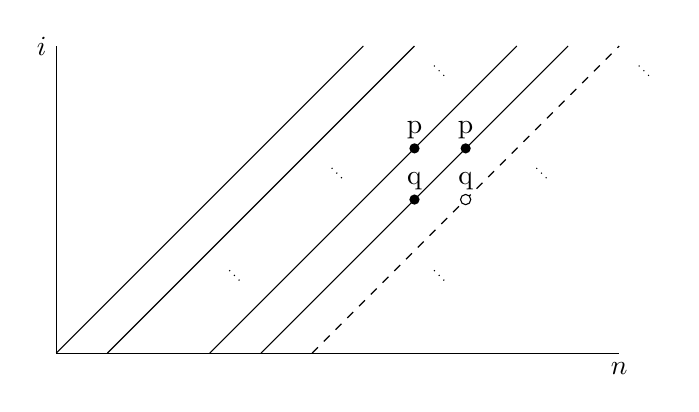
\begin{tikzpicture}[scale = .65]
    \draw (0,0)--(0,6);
    \draw (0,0)--(11,0);
    \draw (0,0)--(6,6);
    \draw (1,0)--(7,6);
    \draw (3,0)--(9,6);
    \draw (4,0)--(10,6);
    \draw[dashed] (5,0)--(11,6);

    \draw[dotted, shorten >=10pt,shorten <=10pt] (3,2)--(4,1);
    \draw[dotted, shorten >=10pt,shorten <=10pt] (5,4)--(6,3);
    \draw[dotted, shorten >=10pt,shorten <=10pt] (7,6)--(8,5);

    \fill (7,4) circle (0.1);
    \fill (8,4) circle (0.1);
    \fill (7,3) circle (0.1);
    \fill[white] (8,3) circle (0.1);
    \draw (8,3) circle (0.1);

    \node[above] at (7,4) {p};
    \node[above] at (8,4) {p};
    \node[above] at (7,3) {q};
    \node[above] at (8,3) {q};

    \draw[dotted, shorten >=10pt,shorten <=10pt] (7,2)--(8,1);
    \draw[dotted, shorten >=10pt,shorten <=10pt] (9,4)--(10,3);
    \draw[dotted, shorten >=10pt,shorten <=10pt] (11,6)--(12,5);

    \node[below] at (11,0) {$n$};
    \node[left] at (0,6) {$i$};
    \end{tikzpicture}
    \caption{Induction step \label{figure}}
\end{figure}

\begin{lemma}
    Let $\{\p(n, i)\}_{n, i}$ and $\{\q(n, i)\}_{n, i}$ each be one of the following two families of propositions:
    \[ \label{proposition: uniqueness: eq1}
    \big\{ \triangle_i (\id_{[n]}) = \Delta_ i(\id_{[n]}) \big\}_{n, i} \qquad
    \big\{ \triangle_i (\id_{[n]}) = T \Delta_ i(\id_{[n]}) \big\}_{n, i.}
    \]
    Then, for $i < n-1$ the following implication holds:
    \[ \label{proposition: uniqueness: eq2}
    \boxed{\p(n,i+1) \wedge \p(n-1,i+1) \wedge \q(n-1,i)}\ \Longrightarrow\ \boxed{\q(n,i)}
    \]
\end{lemma}

\begin{proof}
%        Let $\big\{ \p(n,i) \big\}_{n,i \in \Z}$ and $\big\{ \q(n,i) \big\}_{n,i \in \Z}$ both be the family $\big\{ (\Delta_i)_n = \nabla^{n \choose n-i} \big\}_{n,i \in \Z.}$ The other options are treated analogously.
%
%		From $\p(n, i+1)$ and $\p(n-1, i+1)$ we have
%		\[
%		\partial \triangle_{i+1}(\id_{[n]}) + \triangle_{i+1} (\partial \id_{[n]}) = \partial \Delta_{i+1}(\id_{[n]}) + \Delta_{i+1} (\partial \id_{[n]})
%		\]
%		or, equivalently,
%		\[
%		(1+T) \triangle_{i} (\id_{[n]}) = (1+T) \Delta_{i} (\id_{[n]})
%		\]
%		Lemma \ref{lemma: extra lemma} implies
%		\begin{equation} \label{proposition: uniqueness: induction step: eq1}
%		\Delta_{i}(\id_{[n]}) \ = \!\!\! \sum_{U \in \P_{n-i}(n)} d_{U^{\xi}}(\id_{[n]}) \tensor d_{U^{{\bar{\xi}}}}(\id_{[n]})
%		\end{equation}
%		for some ${\bar{\xi}},\, \xi: \P_{n-i}(n)\to\{+,-\}$. To finish the proof we need to show $\xi(U) = -$ and ${\bar{\xi}}(U) = +$
%		for each $U \in \P_{n-i}(n)$.  Therefore,
%		\[
%		(1+T)\,(\Delta_{i-1})_n =
%		\partial_{n+i}\, (\Delta_{i})_n\ +\ (\Delta_{i})_{n-1}\, \partial_{n}
%		\]
\end{proof}

\begin{proposition} \label{proposition: uniqueness}
    Steenrod's cup-$i$ construction is isomorphic to $\triangle$.
\end{proposition}

\begin{proof}
    content...
\end{proof}

\section{Examples}

\begin{lemma} \label{lemma: free and non-deg in coproduct}
	A cup-$i$ construction $\triangle$ is free if and only if for $i < n$
	\[
	\triangle_i (\id_{[n]}) = \sum_{\Lambda} \sigma^1_\lambda \otimes \sigma^2_\lambda
	\]
	is such that $\sigma^1_\lambda \otimes \sigma^2_\lambda \neq \sigma^2_\mu \otimes \sigma^1_\mu$ for every $\lambda, \mu \in \Lambda$.
\end{lemma}

We now review Steenrod's original cup-$i$ construction \cite{steenrod1947products} pag.  293, see also \cite{mcclure2003multivariable} pag. 682, and prove that it is free and non-degenerate.

\begin{definition}
	\textbf{Steenrod's cup-$i$ construction} $\Delta^{St} : W \to \mathcal{Z}(2)$ is defined by letting $\Delta_i^{St} \big( \id_{[n]} \big)$ be the sum over all sequences
	\[
	0 < p_1 < \cdots < p_{i+1} < n
	\]
	of the basis element
	\begin{equation} \label{equation: steenrod original i odd}
	\begin{split}
	[ 0, \dots, &{p_1} ] \ast [ {p_2}, \dots, {p_3} ] \ast \cdots \ast [ {p_{i+1}}, \dots, n ]\ \tensor \\
	[ &{p_1}, \dots, {p_2} ] \ast \cdots \ast [ {p_{i}}, \dots, {p_{i+1}} ]
	\end{split}
	\end{equation}
	if $i$ is odd, and of
	\begin{equation} \label{equation: steenrod original i even}
	\begin{split}
	[ 0, \dots, &{p_1} ] \ast [ {p_2}, \dots, {p_3} ] \ast \cdots \ast [ {p_{i}}, \dots, {p_{i+1}} ]\ \tensor \\
	[ &{p_1}, \dots, {p_2} ] \ast [ {p_3}, \dots, {p_4} ] \ast \cdots \ast [ {p_{i+1}}, \dots, n ]
	\end{split}
	\end{equation}
	if $i$ is even, where $\ast$ denotes the join of simplices:
	\[
	[{p_{k-1}}, \dots, {p_{k}} ] \ast [ {p_{k+1}}, \dots, p_{k+2}] = [{p_{k-1}}, \dots, p_k, p_{k+1}, \dots, p_{k+2}].
	\]
\end{definition}

\begin{proposition}
	Steenrod's cup-$i$ construction is free and non-degenerate.
\end{proposition}

\begin{proof}
	Steenrod's cup-$i$ construction if non-degenerate since $\Delta_0\big([0]\big) = [0] \otimes [0]$. To prove it is free let us assume $i$ is odd with $i < n$. The $i$ even case is done analogously. Using Lemma \ref{lemma: free and non-deg in coproduct} in a proof by contradiction we can assume that there exist at least two distinct sequences
	\begin{align*}
	\begin{split}
	0 &= p_0 < p_1   < \cdots < p_{i+1} < p_{i+2} = n \\
	0 &= q_0 < q_1 \,<  \cdots < q_{i+1} < q_{i+2} = n
	\end{split}
	\end{align*}
	such that
	\[
	\begin{split}
	&[ {p_0}, \dots, {p_1} ] \ast [ {p_2}, \dots, {p_3} ] \ast \cdots \ast [ {p_{i}}, \dots, {p_{i+1}} ]\ = \\
	&[ {q_1}, \dots, {q_2} ] \ast [ {q_3}, \dots, {q_4} ] \ast \cdots \ast [ {q_{i+1}}, \dots, {q_{i+2}} ]
	\end{split}
	\]
	and
	\[
	\begin{split}
	&[ {q_0}, \dots, {q_1} ] \ast [ {q_2}, \dots, {q_3} ] \ast \cdots \ast [ {q_{i}}, \dots, {q_{i+1}} ]\ = \\
	&[ {p_1}, \dots, {p_2} ] \ast [ {p_3}, \dots, {p_4} ] \ast \cdots \ast [ {p_{i+1}}, \dots, {p_{i+2}} ].
	\end{split}
	\]
	We will prove that $p_{r+1} = q_{r+1} = r$ for $0 \leq r \leq i$, in particular, this will imply the contradiction $i = n$. We have the base case of an induction argument since ${p_0} = {q_1} = {p_0} = {q_1} = 0$. The induction step follows from the identities
	\[
	\begin{split}
	[p_r] &\ast [p_{r+1}] = [q_r, q_{r}+1]\\
	[q_r] &\ast [q_{r+1}] = [p_r, p_{r}+1]
	\end{split}
	\]
	and the lemma is proven.
\end{proof}